% !TEX program = xelatex
% EI conference draft, UTF-8 source.
\documentclass[UTF8,a4paper,10.5pt,fontset=windows]{ctexart}

\usepackage[left=2.1cm,right=2.1cm,top=2.0cm,bottom=2.0cm]{geometry}
\usepackage{amsmath,amssymb}
\usepackage{booktabs}
\usepackage{graphicx}
\usepackage{caption}
\usepackage{float}
\usepackage{xcolor}
\usepackage{hyperref}

\hypersetup{colorlinks=true,linkcolor=blue!60!black,citecolor=blue!60!black,urlcolor=blue!60!black}
\captionsetup[table]{font=small,labelfont=bf,labelsep=quad}
\captionsetup[figure]{font=small,labelfont=bf,labelsep=quad}
\setlength{\parindent}{2em}
\setlength{\parskip}{0.2em}

\title{\textbf{基于原始脑电与眼电可靠性门控融合的驾驶疲劳检测方法}\\[3pt]
\large A Raw EEG-EOG Reliability-Gated Fusion Method for Driver Fatigue Detection}
\author{作者姓名待补充\\单位待补充}
\date{}

\begin{document}
\maketitle

\begin{abstract}
驾驶疲劳检测是智能交通安全中的重要研究问题。SEED-VIG 数据集提供同步采集的脑电（EEG）、眼电（EOG）与连续 PERCLOS 警觉度标签，为基于生理信号的驾驶疲劳检测提供了公开评估平台。针对传统特征方法依赖人工特征、直接多模态拼接容易引入冗余和噪声的问题，本文提出一种基于原始 EEG/EOG 的可靠性门控融合方法。该方法使用轻量 CNN patch encoder 从原始信号中提取窗口级 token 表征，以 EEG 表征作为查询、EOG token 作为键值进行跨模态注意力读取，并通过可靠性门控自适应控制眼电信息的注入强度。考虑到 PERCLOS 是连续警觉度标签，本文将 PERCLOS 回归作为主训练目标，二分类指标由回归输出阈值化得到。在严格 group-subject 跨被试协议下，本文 no-delta 可靠性门控模型达到 Acc 0.8263、Macro-F1 0.8043、Balanced Accuracy 0.8017、RMSE 0.1433 和 Pearson 0.8508，较传统特征拼接和早期原始信号融合模型均有明显提升。消融实验表明，回归目标比 CE-only 更适合连续 PERCLOS 估计，简单时间差分模块在当前设置下并不稳定，适合作为消融项而非主模块。

\noindent\textbf{关键词：}驾驶疲劳检测；脑电；眼电；PERCLOS；跨模态注意力；可靠性门控；跨被试评估
\end{abstract}

\begin{abstract}
\noindent\textbf{Abstract:} Driver fatigue detection is an important problem in intelligent transportation safety. The SEED-VIG dataset provides synchronized EEG, EOG, and continuous PERCLOS vigilance labels for physiological fatigue detection. To reduce dependence on handcrafted features and avoid redundant naive multimodal concatenation, this paper proposes a raw EEG-EOG reliability-gated fusion method. Lightweight CNN patch encoders extract window-level token representations from raw EEG and EOG. EEG representations query EOG tokens through cross-modal attention, and a reliability gate adaptively controls the contribution of ocular evidence. Since PERCLOS is continuous, regression is used as the main objective, and binary metrics are computed by thresholding the regression output. Under a strict group-subject protocol, the proposed no-delta reliability-gated model achieves Acc 0.8263, Macro-F1 0.8043, Balanced Accuracy 0.8017, RMSE 0.1433, and Pearson 0.8508. Ablation results show that regression is more suitable than CE-only for continuous PERCLOS estimation, while the simple temporal delta module is unstable in the current setting and should be treated as an ablation component.

\noindent\textbf{Keywords:} driver fatigue detection; EEG; EOG; PERCLOS; cross-modal attention; reliability gate; cross-subject evaluation
\end{abstract}

\section{引言}
驾驶疲劳会降低驾驶员的注意力、反应速度和风险感知能力，是交通事故的重要诱因。基于生理信号的疲劳检测能够从驾驶员内部状态出发刻画疲劳变化，其中 EEG 反映神经活动状态，EOG 记录眨眼、眼睑闭合和眼球运动等行为变化，两者在驾驶疲劳检测中具有互补价值。SEED-VIG 数据集通过模拟驾驶任务同步采集 EEG、EOG 与眼动信息，并以 PERCLOS 作为连续警觉度标签，是该方向常用公开数据集之一\cite{seedvig,zheng2017}。

已有研究表明，多模态 EEG/EOG 融合能够提升警觉度估计效果\cite{zheng2017}。近期 HMS-TENet 使用分频段 EEG/EOG 特征、多尺度结构和拓扑注意力进行驾驶警觉度估计\cite{hmstenet2024}；GE-LSTM-Net 则强调 EEG 时空特征中的全局--局部依赖建模\cite{gelstm2026}。这些工作说明，跨模态信息融合、时空建模和跨被试泛化是驾驶疲劳检测中的关键问题。

然而，SEED-VIG 的 PERCLOS 标签与眼部闭合直接相关，EOG 在该数据集上天然具有较强预测能力。因此，多模态模型不能只报告相对 EEG-only 或传统特征模型的提升，还需要在严格跨被试协议下说明融合模块的实际收益和边界。为此，本文直接使用原始 EEG/EOG 信号，构建可靠性门控融合模型，并将连续 PERCLOS 回归作为主任务，分类指标仅作为阈值化后的工程指标。

本文主要贡献如下：
\begin{enumerate}
  \item 提出一种面向原始 EEG/EOG 信号的可靠性门控融合框架，减少人工特征依赖；
  \item 设计 EEG-query/EOG-key-value 跨模态注意力，使 EEG 表征按需读取眼动证据；
  \item 将连续 PERCLOS 回归作为主训练目标，并通过消融证明 CE-only 不适合作为连续警觉度估计主目标；
  \item 在严格 group-subject 协议下系统比较传统特征、早期 raw fusion、时间差分和强基线，给出保守且可复现的实验结论。
\end{enumerate}

\section{方法}
\subsection{输入窗口与原始信号编码}
模型以 8 个连续 8 秒窗口作为一个样本，总时长约 64 秒。EEG 输入维度为 $[B,8,17,1600]$，其中 17 表示 EEG 通道数，1600 对应 $8\text{s}\times200\text{Hz}$；EOG 输入维度为 $[B,8,7,1000]$，其中 7 表示 EOG 通道数，1000 对应 $8\text{s}\times125\text{Hz}$。

两路信号分别经过独立 CNN patch encoder 提取 token 表征。EEG 分支进一步使用轻量 window Transformer 建模窗口内 token 关系，并池化为窗口级表示；EOG 分支保留 token 序列，作为后续跨模态注意力中的 Key 和 Value。该设计避免过早压缩 EOG token，使注意力模块仍能在眼动局部片段中选择有效证据。

\subsection{跨模态注意力}
对于每个时间窗口，模型以 EEG 窗口表示作为 Query，以 EOG token 作为 Key 和 Value 计算跨模态注意力：
\begin{equation}
E_{att}=\mathrm{softmax}\left(\frac{QK^\top}{\sqrt{d_k}}\right)V .
\end{equation}
该过程使 EEG 表征根据当前脑电上下文，从 EOG token 中读取相关眼动证据，而不是将两种模态进行无差别拼接。

\subsection{可靠性门控融合}
EOG 既包含闭眼、眨眼等疲劳相关信息，也可能包含自主眼动或瞬时扰动。为控制 EOG 信息注入强度，本文使用门控网络根据 EEG 表征与注意力读取到的 EOG 表征输出可靠性权重：
\begin{equation}
g=\sigma(W_2\,\mathrm{GELU}(W_1[E_{EEG};E_{att}])) .
\end{equation}
最终融合表示为
\begin{equation}
H=\mathrm{LayerNorm}(E_{EEG}+g\odot E_{att}) .
\end{equation}
其中 $g$ 是窗口级 EOG 可靠性权重。跨模态注意力负责在 EOG token 中选择相关证据，门控机制负责判断该证据是否应进入融合表示，两者功能互补。

\subsection{时序建模与训练目标}
融合后的 8 个窗口表示加入位置编码，并输入一层 temporal Transformer 建模窗口间变化。本文主模型不使用 temporal delta；该模块仅作为消融项保留。模型主输出为连续 PERCLOS 估计值，训练损失为
\begin{equation}
L_{reg}=\mathrm{SmoothL1}(\hat{y}, y_{perclos}) .
\end{equation}
二分类指标由回归输出按阈值 0.35 映射得到。CE-only 和分类--回归多任务训练仅用于消融实验。

\begin{figure}[H]
  \centering
  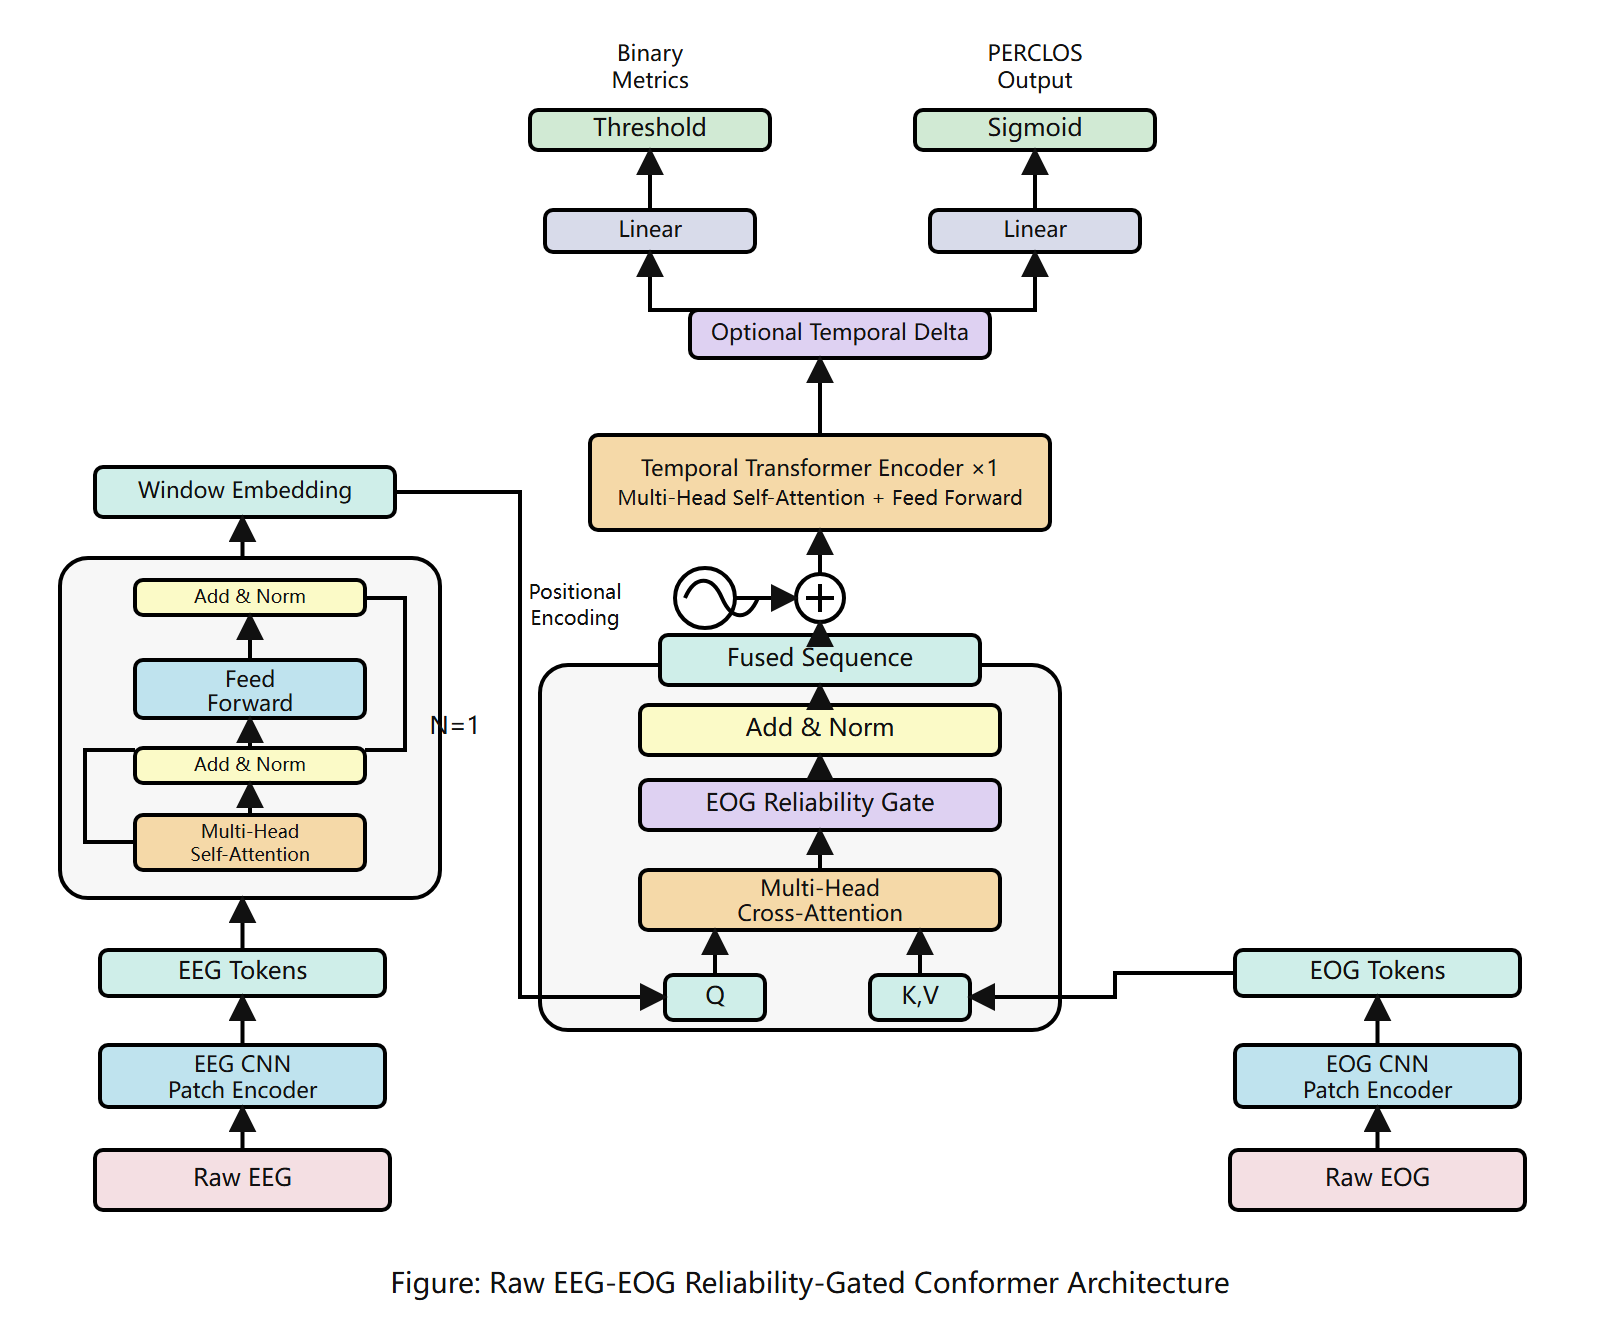
\includegraphics[width=0.88\linewidth]{raw_eeg_eog_reliability_gated_conformer_cn.png}
  \caption{原始 EEG/EOG 可靠性门控融合模型结构。PERCLOS 回归是主输出，二分类结果由阈值化得到；Temporal Delta 仅作为消融模块。}
  \label{fig:arch}
\end{figure}

\section{实验设置}
\subsection{数据集与评估协议}
实验基于 SEED-VIG 数据集。该数据集在模拟驾驶任务中采集 EEG、EOG 和眼动信息，并提供连续 PERCLOS 警觉度标签\cite{seedvig,zheng2017}。本文每 8 秒构造一个窗口，连续 8 个窗口组成一个样本。

本文主结果采用 group-subject 5 折协议，即训练集和测试集按被试划分，保证测试被试不出现在训练集中。该协议比同实验内随机划分更能反映跨被试泛化能力。

\subsection{评价指标与训练设置}
连续 PERCLOS 估计使用 RMSE 和 Pearson 相关系数评价。二分类指标包括 Accuracy、Macro-F1 与 Balanced Accuracy，由回归输出阈值化得到。模型训练 20 epoch，batch size 为 4，优化器为 AdamW。

\section{实验结果与分析}
\subsection{主结果}
表~\ref{tab:main} 给出严格 group-subject 协议下的主结果。与传统特征拼接和早期 raw cross-attention 相比，可靠性门控融合明显提高跨被试表现。no-delta 版本在分类工程指标上取得最高 Acc、F1 和 Balanced Accuracy，回归指标也接近强基线。

\begin{table}[H]
\centering
\caption{主结果（group-subject, binary, 5 折均值）。}
\label{tab:main}
\resizebox{\linewidth}{!}{
\begin{tabular}{lcccccc}
\toprule
方法 & 训练目标 & Acc$\uparrow$ & F1$\uparrow$ & BalAcc$\uparrow$ & RMSE$\downarrow$ & Pearson$\uparrow$ \\
\midrule
传统特征拼接 & -- & 0.4912 & -- & -- & 0.2563 & 0.5746 \\
Raw EEG/EOG Cross-Attention & regression & 0.7233 & 0.7241 & 0.7332 & 0.1652 & 0.8145 \\
Delta/Gate & regression & 0.8233 & 0.7995 & 0.7977 & 0.1483 & 0.8406 \\
Anchor Residual + Delta & regression & 0.8027 & 0.7894 & 0.7993 & 0.1471 & 0.8398 \\
Reliability-Gated No-Delta & regression & \textbf{0.8263} & \textbf{0.8043} & \textbf{0.8017} & 0.1433 & 0.8508 \\
EOG-only strong baseline & regression & 0.8250 & 0.7883 & 0.7820 & \textbf{0.1432} & \textbf{0.8536} \\
\bottomrule
\end{tabular}}
\end{table}

结果表明，本文方法不能被表述为在所有 clean average 指标上全面超过 EOG-only 强基线；更准确的结论是：可靠性门控融合在连续回归指标上达到接近强基线的性能，在 F1 与 Balanced Accuracy 上取得更高结果，并显著优于传统特征和早期原始信号融合方法。

\subsection{训练目标消融}
表~\ref{tab:objective} 比较 CE-only 与 regression-only。CE-only 能直接优化二分类指标，但会显著破坏连续 PERCLOS 估计，RMSE 升至 0.30 以上且 Pearson 为负。因此，本文将 regression-only 固定为主方法，分类损失仅作为消融对照。

\begin{table}[H]
\centering
\caption{训练目标消融（group-subject, binary, 5 折均值）。}
\label{tab:objective}
\resizebox{0.95\linewidth}{!}{
\begin{tabular}{llccccc}
\toprule
模型 & 目标 & Acc & F1 & BalAcc & RMSE & Pearson \\
\midrule
EOG-only & classification & 0.8261 & 0.8118 & 0.8191 & 0.3070 & -0.4279 \\
Delta-Gate & classification & 0.8080 & 0.7926 & 0.8020 & 0.3105 & -0.7082 \\
EOG-only & regression & 0.8250 & 0.7883 & 0.7820 & 0.1432 & 0.8536 \\
Delta-Gate & regression & 0.8233 & 0.7995 & 0.7977 & 0.1483 & 0.8406 \\
\bottomrule
\end{tabular}}
\end{table}

\subsection{划分协议影响}
表~\ref{tab:split} 比较 within-experiment 与 group-subject。within-experiment 下结果更高，但可能高估实际跨被试泛化能力。本文将 group-subject 作为主协议，更符合真实部署中面对新驾驶员的场景。

\begin{table}[H]
\centering
\caption{划分协议影响（EEG+EOG cross-attention, 3-class, 5 折均值）。}
\label{tab:split}
\begin{tabular}{lccccc}
\toprule
协议 & Acc & F1 & BalAcc & RMSE & Pearson \\
\midrule
within-experiment & 0.7732 & 0.7700 & 0.7802 & 0.1320 & 0.8637 \\
group-subject seed0 & 0.7233 & 0.7241 & 0.7332 & 0.1652 & 0.8145 \\
group-subject seed1 & 0.7068 & 0.7098 & 0.7143 & 0.1533 & 0.8370 \\
\bottomrule
\end{tabular}
\end{table}

\subsection{鲁棒性讨论}
在初步 EOG 退化测试中，部分随机 mask 场景下融合模型仍不够稳定；但在严重 EOG 缺失设置下，融合模型仍保持可用预测能力（EOG 全零场景 RMSE 为 0.3394）。这说明 EEG 分支的价值更适合表述为退化保护和困难样本补偿，而不是 clean average 指标上的全面领先。后续投稿版本可进一步补充完整的 EOG 退化表格。

\section{讨论}
本文的核心叙事是“原始 EEG/EOG 可靠性门控融合与严格跨被试评估”。该叙事避免将 temporal delta 作为未经充分证明的核心创新，也避免把分类准确率作为唯一目标。实验显示，PERCLOS 连续估计更适合使用回归损失；同时，由于 EOG 与 PERCLOS 标签天然相关，多模态融合的价值应结合公平强基线和鲁棒性场景进行解释。

本文仍存在局限。首先，当前模型在 clean average 回归指标上未显著超过 EOG-only 强基线，因此不能夸大平均性能优势。其次，EOG 部分缺失和随机 mask 场景下的融合稳定性仍需提升。最后，跨被试个体差异明显，未来可进一步引入 subject-invariant 表征学习或轻量校准策略。

\section{结论}
本文提出一种基于原始 EEG/EOG 的可靠性门控融合方法，用于 SEED-VIG 数据集上的驾驶疲劳检测与连续 PERCLOS 警觉度估计。模型通过 EEG-query/EOG-key-value 跨模态注意力读取眼动证据，并使用门控机制控制 EOG 信息注入。实验表明，在严格 group-subject 协议下，no-delta 可靠性门控模型达到 Acc 0.8263、F1 0.8043、RMSE 0.1433 和 Pearson 0.8508，较传统特征和早期 raw fusion 明显提升。消融结果进一步说明，回归目标比 CE-only 更适合 PERCLOS 连续估计，Temporal Delta 当前不宜作为主模块。

\begin{thebibliography}{9}
\bibitem{zheng2017}
Zheng W.-L., Lu B.-L. A multimodal approach to estimating vigilance using EEG and forehead EOG. \textit{Journal of Neural Engineering}, 14(2):026017, 2017.

\bibitem{seedvig}
SEED-VIG Dataset. Brain-like Computing and Machine Intelligence Lab, Shanghai Jiao Tong University. \url{https://bcmi.sjtu.edu.cn/home/seed/seed-vig.html}

\bibitem{hmstenet2024}
Tang M., Li P., Zhang H., Deng L., Liu S., Zheng Q., Gao D. HMS-TENet: A hierarchical multi-scale topological enhanced network based on EEG and EOG for driver vigilance estimation. \textit{Biomedical Technology}, 8:92--103, 2024. DOI: 10.1016/j.bmt.2024.10.003.

\bibitem{gelstm2026}
Lan H., Tang M., Ju X., Li M., Hu D. GE-LSTM-Net: A global-enhanced LSTM network with attention for spatiotemporal feature extraction in EEG-based vigilance estimation. \textit{CAAI Artificial Intelligence Research}, 5:9150001, 2026. DOI: 10.26599/AIR.2026.9150001.
\end{thebibliography}

\end{document}
